% THIS IS SIGPROC-SP.TEX - VERSION 3.0
% WORKS WITH V3.1SP OF ACM_PROC_ARTICLE-SP.CLS
% JUNE 2007
%
% It is an example file showing how to use the 'acm_proc_article-sp.cls' V3.1SP
% LaTeX2e document class file for Conference Proceedings submissions.
% ----------------------------------------------------------------------------------------------------------------
% This .tex file (and associated .cls V3.1SP) *DOES NOT* produce:
%       1) The Permission Statement
%       2) The Conference (location) Info information
%       3) The Copyright Line with ACM data
%       4) Page numbering
% ---------------------------------------------------------------------------------------------------------------
% It is an example which *does* use the .bib file (from which the .bbl file
% is produced).
% REMEMBER HOWEVER: After having produced the .bbl file,
% and prior to final submission,
% you need to 'insert'  your .bbl file into your source .tex file so as to provide
% ONE 'self-contained' source file.
%
% Questions regarding SIGS should be sent to
% Adrienne Griscti ---> griscti@acm.org
%
% Questions/suggestions regarding the guidelines, .tex and .cls files, etc. to
% Gerald Murray ---> murray@acm.org
%
% For tracking purposes - this is V3.0SP - JUNE 2007

\documentclass{fp035-thummalapenta}
\pdfpagewidth=8.5in
\pdfpageheight=11in
\usepackage{times}
\usepackage{graphicx}
\usepackage{epsf}
\usepackage{verbatim}
\usepackage{psfig}
\usepackage{cite}
\usepackage{url}
\usepackage{color}
\usepackage{alltt}

\usepackage{longtable,lscape}
\usepackage{slashbox,multirow}
\usepackage{colortbl}
\usepackage{mathrsfs}

\newcommand{\Add}{\CodeIn{add}}
\newcommand{\AVTree}{\CodeIn{AVTree}}
\newcommand{\Assignment}[3]{$\langle$ \Object{#1}, \Object{#2}, \Object{#3} $\rangle$}
\newcommand{\BinaryTreeRemove}{\CodeIn{BinaryTree\_remove}}
\newcommand{\BinaryTree}{\CodeIn{BinaryTree}}
\newcommand{\Caption}{\caption}
\newcommand{\Char}[1]{`#1'}
\newcommand{\CheckRep}{\CodeIn{checkRep}}
\newcommand{\ClassC}{\CodeIn{C}}
\newcommand{\CodeIn}[1]{{\small\texttt{#1}}}
\newcommand{\CodeOutSize}{\scriptsize}
\newcommand{\Comment}[1]{}
\newcommand{\Ensures}{\CodeIn{ensures}}
\newcommand{\ExtractMax}{\CodeIn{extractMax}}
\newcommand{\FAL}{field-ordering}
\newcommand{\FALs}{field-orderings}
\newcommand{\Fact}{observation}
\newcommand{\Get}{\CodeIn{get}}
\newcommand{\HashSet}{\CodeIn{HashSet}}
\newcommand{\HeapArray}{\CodeIn{HeapArray}}
\newcommand{\Intro}[1]{\emph{#1}}
\newcommand{\Invariant}{\CodeIn{invariant}}
\newcommand{\JUC}{\CodeIn{java.\-util.\-Collections}}
\newcommand{\JUS}{\CodeIn{java.\-util.\-Set}}
\newcommand{\JUTM}{\CodeIn{java.\-util.\-TreeMap}}
\newcommand{\JUTS}{\CodeIn{java.\-util.\-TreeSet}}
\newcommand{\JUV}{\CodeIn{java.\-util.\-Vector}}
\newcommand{\JMLPlusJUnit}{JML+JUnit}
\newcommand{\Korat}{Korat}
\newcommand{\Left}{\CodeIn{left}}
\newcommand{\Lookup}{\CodeIn{lookup}}
\newcommand{\MethM}{\CodeIn{m}}
\newcommand{\Node}[1]{\CodeIn{N}$_#1$}
\newcommand{\Null}{\CodeIn{null}}
\newcommand{\Object}[1]{\CodeIn{o}\ensuremath{_#1}}
\newcommand{\PostM}{\MethM$_{post}$}
\newcommand{\PreM}{\MethM$_{pre}$}
\newcommand{\Put}{\CodeIn{put}}
\newcommand{\Remove}{\CodeIn{remove}}
\newcommand{\RepOk}{\CodeIn{repOk}}
\newcommand{\Requires}{\CodeIn{requires}}
\newcommand{\Reverse}{\CodeIn{reverse}}
\newcommand{\Right}{\CodeIn{right}}
\newcommand{\Root}{\CodeIn{root}}
\newcommand{\Set}{\CodeIn{set}}
\newcommand{\State}[1]{2^{#1}}
\newcommand{\TestEra}{TestEra}
\newcommand{\TreeMap}{\CodeIn{TreeMap}}

\newenvironment{CodeOut}{\begin{scriptsize}}{\end{scriptsize}}
\newenvironment{SmallOut}{\begin{small}}{\end{small}}

\newcommand{\pairwiseEquals}{PairwiseEquals}
\newcommand{\monitorEquals}{MonitorEquals}
%\newcommand{\monitorWField}{WholeStateW}
\newcommand{\traverseField}{WholeState}
\newcommand{\monitorSMSeq}{ModifyingSeq}
\newcommand{\monitorSeq}{WholeSeq}

\newcommand{\IntStack}{\CodeIn{IntStack}}
\newcommand{\UBStack}{\CodeIn{UBStack}}
\newcommand{\BSet}{\CodeIn{BSet}}
\newcommand{\BBag}{\CodeIn{BBag}}
\newcommand{\ShoppingCart}{\CodeIn{ShoppingCart}}
\newcommand{\BankAccount}{\CodeIn{BankAccount}}
\newcommand{\BinarySearchTree}{\CodeIn{BinarySearchTree}}
\newcommand{\LinkedList}{\CodeIn{LinkedList}}

\newcommand{\Book}{\CodeIn{Book}}
\newcommand{\Library}{\CodeIn{Library}}

\newcommand{\Jtest}{Jtest}
\newcommand{\JCrasher}{JCrasher}
\newcommand{\Daikon}{Daikon}
\newcommand{\JUnit}{JUnit}

\newcommand{\trie}{trie}

\newcommand{\Perl}{Perl}


\newcommand{\SubjectCount}{11}
\newcommand{\DSSubjectCount}{two}

\newcommand{\Equals}{\CodeIn{equals}}
\newcommand{\Pairwise}{PairwiseEquals}
\newcommand{\Subgraph}{MonitorEquals}
\newcommand{\Concrete}{WholeState}
\newcommand{\ModSeq}{ModifyingSeq}
\newcommand{\Seq}{WholeSeq}
\newcommand{\Aeq}{equality}

\newcommand{\Meaning}[1]{\ensuremath{[\![}#1\ensuremath{]\!]}}
\newcommand{\Pair}[2]{\ensuremath{\langle #1, #2 \rangle}}
\newcommand{\Triple}[3]{\ensuremath{\langle #1, #2, #3 \rangle}}
\newcommand{\SetSuch}[2]{\ensuremath{\{ #1 | #2 \}}}

\newcommand{\Equiv}[2]{\ensuremath{#1 \EquivSTRel{} #2}}
\newcommand{\EquivME}{\Equiv}
\newcommand{\EquivST}{\Equiv}
\newcommand{\EquivSTRel}{\ensuremath{\cong}}
\newcommand{\Redundant}[2]{\ensuremath{#1 \lhd #2}}
\newcommand{\VB}{\ensuremath{\mid}}
\newcommand{\MES}{method-entry state}

\newcommand{\Small}[1]{{\small{#1}}}

\newcommand{\CenterCell}[1]{\multicolumn{1}{c|}{#1}}

%-- Begin patch area for accents in 'Author Block' area - may be needed by some authors / but not all
\DeclareFixedFont{\auacc}{OT1}{phv}{m}{n}{12}   % Needed for "Author Block" accents - Patch by Gerry 3/21/07
\DeclareFixedFont{\afacc}{OT1}{phv}{m}{n}{10}   % Needed for "Author Block" accents in the affiliation/address line - Patch by Gerry 3/21/07
%--
\begin{document}
\conferenceinfo{ASE'07,} {November 4--9, 2007, Atlanta, Georgia, USA.}
\CopyrightYear{2007}
\crdata{978-1-59593-882-4/07/0011}

\title{PARSEWeb: A Programmer Assistant for Reusing Open Source Code on the Web}

%
% You need the command \numberofauthors to handle the 'placement
% and alignment' of the authors beneath the title.
%
% For aesthetic reasons, we recommend 'three authors at a time'
% i.e. three 'name/affiliation blocks' be placed beneath the title.
%
% NOTE: You are NOT restricted in how many 'rows' of
% "name/affiliations" may appear. We just ask that you restrict
% the number of 'columns' to three.
%
% Because of the available 'opening page real-estate'
% we ask you to refrain from putting more than six authors
% (two rows with three columns) beneath the article title.
% More than six makes the first-page appear very cluttered indeed.
%
% Use the \alignauthor commands to handle the names
% and affiliations for an 'aesthetic maximum' of six authors.
% Add names, affiliations, addresses for
% the seventh etc. author(s) as the argument for the
% \additionalauthors command.
% These 'additional authors' will be output/set for you
% without further effort on your part as the last section in
% the body of your article BEFORE References or any Appendices.

\numberofauthors{2} %  in this sample file, there are a *total*
% of EIGHT authors. SIX appear on the 'first-page' (for formatting
% reasons) and the remaining two appear in the \additionalauthors section.
%
\author{
% You can go ahead and credit any number of authors here,
% e.g. one 'row of three' or two rows (consisting of one row of three
% and a second row of one, two or three).
%
% The command \alignauthor (no curly braces needed) should
% precede each author name, affiliation/snail-mail address and
% e-mail address. Additionally, tag each line of
% affiliation/address with \affaddr, and tag the
% e-mail address with \email.
%
% 1st. author
\alignauthor
Suresh Thummalapenta\\
       \affaddr{Department of Computer Science}\\
       \affaddr{North Carolina State University}\\
       \affaddr{Raleigh, USA}\\
       \email{sthumma@ncsu.edu}
% 2nd. author
\alignauthor
Tao Xie\\
\affaddr{Department of Computer Science}\\
       \affaddr{North Carolina State University}\\
       \affaddr{Raleigh, USA}\\
       \email{xie@csc.ncsu.edu}
}
\maketitle

\begin{abstract}

Programmers commonly reuse existing frameworks or libraries to
reduce software development efforts. One common problem in reusing
the existing frameworks or libraries is that the programmers know what type
of object that they need, but do not know how to get that object
with a specific method sequence. To help programmers to address this
issue, we have developed an approach that takes queries of the form
``Source object type $\rightarrow$ Destination object type'' as
input, and suggests relevant method-invocation sequences that can
serve as solutions that yield the destination object from the source object 
given in the query. Our approach interacts with
a code search engine (CSE) to gather relevant code samples and
performs static analysis over the gathered samples to extract
required sequences. As code samples are collected on demand through
CSE, our approach is not limited to queries of any specific set of frameworks
or libraries. We have implemented our approach with a tool called
PARSEWeb, and conducted four different evaluations to show that our
approach is effective in addressing programmers' queries. We also
show that PARSEWeb performs better than existing related tools:
Prospector and Strathcona.

\end{abstract}

\vspace{1mm} \noindent {\bf Categories and Subject Descriptors:}
D.2.3 {[Software Engineering]}: {Coding Tools and
Techniques---\emph{Object-oriented programming}}; D.2.6 {[Software Engineering]}: {Programming
Environments---\emph{Integrated environments}};

\vspace{1mm} \noindent {\bf General Terms:} Languages,
Experimentation.

\vspace{1mm} \noindent {\bf Keywords:} Code reuse, Code search
engine, Code examples, Ranking code samples

%-------------------------------------------------------------------------
\section{Introduction}
\label{sec:introduction}

The primary goal of software development is to deliver high-quality
software efficiently and in the least amount of time whenever
possible. To achieve the preceding goal, programmers often want to
reuse existing frameworks or libraries instead of developing similar
code artifacts from scratch. The challenging aspect for
programmers in reusing the existing frameworks or libraries is to
understand the usage of Application Programming Interfaces (APIs)
exposed by those frameworks or libraries, because many of the
existing frameworks or libraries are not well-documented. Even when
such documentations exist, they are often outdated~\cite{document:leth}.

In general, the reuse of existing frameworks or libraries involve
instantiation of several object types of those frameworks or
libraries. For example, consider the programming task of parsing
code in a dirty editor (editor whose content is not yet saved) of
the Eclipse IDE framework. As a dirty editor is represented as an
object of the \CodeIn{IEditorPart} type and the programmer needs an
object of \CodeIn{ICompilationUnit} for parsing, the programmer has
to identify a method sequence that takes the \CodeIn{IEditorPart} object
as input and results in an object of \CodeIn{ICompilationUnit}. One
such possible method sequence is shown below:

\begin{CodeOut}
\begin{alltt}
IEditorPart iep = ...
IEditorInput editorInp = iep.getEditorInput();
IWorkingCopyManager wcm = JavaUI.getWorkingCopyManager();
ICompilationUnit icu = wcm.getWorkingCopy(editorInp);
\end{alltt}
\end{CodeOut}

The code sample shown above exhibits the difficulties faced by
programmers in reusing the existing frameworks or libraries. A
programmer unfamiliar to Eclipse may take
long time to identify that an \CodeIn{IWorkingCopyManager} object 
is needed for getting the
\CodeIn{ICompilationUnit} object from an object of the
\CodeIn{IEditorInput} type. Furthermore, it is not trivial to find
an appropriate way of instantiating the
\CodeIn{IWorkingCopyManager} object as the instantiation requires a static
method invocation on the \CodeIn{JavaUI} class.

In many such situations, programmers know what type of object that
they need to instantiate (like \CodeIn{ICompilationUnit}), but do
not know how to write code to get that object from a known object
type (like \CodeIn{IEditorPart}). For simplicity, we refer the known
object type as \emph{Source} and the required object type as
\emph{Destination}. Therefore, the proposed problem can be
translated to a query of the form ``\emph{Source} $\rightarrow$
\emph{Destination}''. There are several existing
approaches~\cite{prospector:jungloid, strathcona:se, xsnippet:saha}
that address the described problem. But the common issue faced by
these existing approaches is that the scope of these approaches is
limited to the information available in a fixed (often small) set of
applications reusing the frameworks or libraries of interest.
%-------------------------------------------------------------------------
\begin{figure*}[t]
\begin{CodeOut}
\begin{alltt}
\hspace*{0.6in}01:\textbf{FileName}:0\_UserBean.java \textbf{MethodName}:ingest  \textbf{Rank}:1 \textbf{NumberOfOccurrences}:6
\hspace*{0.6in}02:QueueConnectionFactory,createQueueConnection() \textbf{ReturnType}:QueueConnection
\hspace*{0.6in}03:QueueConnection,createQueueSession(boolean,Session.AUTO\_ACKNOWLEDGE) \textbf{ReturnType}:QueueSession
\hspace*{0.6in}04:QueueSession,createSender(Queue) \textbf{ReturnType}:QueueSender
\end{alltt}
\end{CodeOut}
\vspace*{-4ex} \Caption{\label{fig:sampleoutput} Method sequence
suggested by PARSEWeb.}
%-------------------------------------------------------------------------
%\begin{figure}[t]
\begin{CodeOut}
\begin{alltt}
\hspace*{0.6in}01:QueueConnectionFactory qcf;
\hspace*{0.6in}02:QueueConnection queueConn = qcf.createQueueConnection();
\hspace*{0.6in}03:QueueSession qs = queueConn.createQueueSession(true,Session.AUTO\_ACKNOWLEDGE);
\hspace*{0.6in}04:QueueSender queueSender = qs.createSender(new Queue());
\end{alltt}
\end{CodeOut}\vspace*{-4ex}
\Caption{\label{fig:javacode} Equivalent Java code for the method sequence suggested by PARSEWeb.} \vspace*{-3ex}
\end{figure*}
%-------------------------------------------------------------------------
Many code search engines (CSE) such as Google~\cite{GCSE} and
Koders~\cite{KODERS}\Comment{, and Krugle~\cite{KRUGLE}} are
available on the web. These CSEs can be used to assist programmers
by providing relevant code examples with usages of the given query
from a large number of publicly accessible source code repositories.
For the preceding example, programmers can issue the query
``\CodeIn{IEditorPart} \CodeIn{ICompilationUnit}'' to gather
relevant code samples with usages of the object types
\CodeIn{IEditorPart} and \CodeIn{ICompilationUnit}. However, these
CSEs are not quite helpful in addressing the described problem
because we observed that Google Code Search Engine (GCSE)
~\cite{GCSE} returns nearly $100$ results for this
query and the desired method sequence shown above is present in the
$25^{th}$ source file among those results.

Our approach addresses the described problem by accepting
queries of the form ``\emph{Source} $\rightarrow$
\emph{Destination}'' and suggests frequently used Method-Invocation
Sequences (MIS) that can transform an object of the \emph{Source}
type to an object of the \emph{Destination} type. Our approach also
suggests relevant code samples that are extracted from a large
number of publicly accessible source code repositories. These
suggested MISs along with the code samples can help programmers in
addressing the described problem and thereby help reduce
programmers' effort in reusing existing frameworks or libraries.

We have implemented the proposed approach with a tool called
PARSEWeb for helping reuse Java code. PARSEWeb interacts with
GCSE~\cite{GCSE} to search for code samples with the usages of the
given \emph{Source} and \emph{Destination} object types, and
downloads the code example results to form a local source code
repository. PARSEWeb analyzes the local source code repository to
extract different MISs and clusters similar MISs using a
sequence postprocessor. These extracted MISs can serve as a solution for
the given query. PARSEWeb also sorts the final set of MISs using
several ranking heuristics. PARSEWeb uses an additional heuristic
called query splitting that helps address the problem where
code samples for the given query are split among different source
files.

This paper makes the following main contributions:\vspace*{-1ex}
\begin{itemize}
\item An approach for reducing programmers' effort while reusing existing frameworks or libraries by providing frequently used MISs and relevant code samples.
\item A technique for collecting relevant code samples dynamically from the web. This contribution has an added advantage of not limiting the scope of the approach to any specific set of frameworks or libraries.
\item A technique for analyzing partial code samples through Abstract Syntax Trees (AST) and Directed Acyclic Graphs (DAG) that can handle control-flow information and method inlining.
\item An Eclipse plugin tool implemented for the proposed approach
and several evaluations to assess the effectiveness of the tool.
\end{itemize}

The rest of the paper is organized as follows. Section
~\ref{sec:example} explains the approach through an example.
Section~\ref{sec:relatedwork} presents related work.
Section~\ref{sec:summary} describes key aspects of the approach.
Section~\ref{sec:implementation} describes implementation details.
Section~\ref{sec:evaluation} discusses evaluation results.
Section~\ref{sec:discussion} discusses limitations and future work.
Finally, Section~\ref{sec:conclusion} concludes.\vspace*{-1ex}
%-------------------------------------------------------------------------
\section{Example}
\label{sec:example}
We next use an example to illustrate our approach and how our
approach can help in reducing programmers' effort when reusing
existing frameworks or libraries. We use object types
\CodeIn{QueueConnectionFactory} and \CodeIn{QueueSender} from the
OpenJMS library\footnote{\url{http://java.sun.com/products/jms}},
which is an open source implementation of Sun's Java Message Service
API 1.1 Specification. \Comment{This library can be used to send and receive
messages in both synchronous and asynchronous modes. }Consider that a
programmer has an object of type \CodeIn{QueueConnectionFactory} and
does not know how to write code to get a \CodeIn{QueueSender}
object, which is required for sending messages.

To address the problem, the programmer can use our PARSEWeb tool
(implemented for our approach) in the following way. The
programmer first translates the problem into
a ``\CodeIn{QueueConnectionFactory} $\rightarrow$
\CodeIn{QueueSender}'' query. Given this query, PARSEWeb
requests GCSE for relevant code samples with usages of the given
\emph{Source} and \emph{Destination} object types, and downloads the
code samples to form a local source code repository. The downloaded
code samples are often partial and not compilable as GCSE retrieves
(and subsequently PARSEWeb downloads) only source files with usages
of the given object types instead of entire projects. PARSEWeb
analyzes each partial code sample using an Abstract Syntax Tree
(AST) and builds a Directed Acyclic Graph (DAG) that represents each
given code sample in order to capture control-flow information in
the code example. PARSEWeb traverses this DAG to extract MISs that
take \CodeIn{QueueConnectionFactory} as input and result
in an object of \CodeIn{QueueSender}. The output of
PARSEWeb for the given query is shown in Figure~\ref{fig:sampleoutput}.
The sequence starts with the invocation of
the \CodeIn{createQueueConnection} method that results in
an instance of \CodeIn{QueueConnection} type. Similarly, by following
other method invocations, the method sequence finally results in the
\CodeIn{QueueSender} object, which is the desired
destination object of the given query.

The sample output also shows additional details 
such as \CodeIn{FileName}, \CodeIn{MethodName}, \CodeIn{Rank}, and \CodeIn{NumberOfOccurrences}. 
The details \CodeIn{FileName} and
\CodeIn{MethodName} indicate the source file that the programmer can
browse to find a relevant code sample for this MIS. For example, a
code sample of the given query can be found in method
\CodeIn{ingest} of file \CodeIn{0\_UserBean.java}. The prefix of the
file name gives the index of the source file that contained the
suggested solution among the results of GCSE. In this example, the
code sample for the suggested method-invocation sequence can be
found in the first source file returned by GCSE as the prefix value
is zero. Generally, many queries result in more than one possible
solution. The \CodeIn{Rank} attribute gives the rank of the
corresponding MIS among the complete set of results. PARSEWeb
derives the rank of a MIS based on the \CodeIn{NumberOfOccurrences}
attribute and some other heuristics described in
Section~\ref{sec:rankingCriteria}. The suggested MIS contains all
necessary information for the programmer to write code for getting
the \emph{Destination} object from the given \emph{Source} object.
The suggested MIS can be transformed to equivalent Java code by
introducing required intermediate variables. The code sample
suggested along with the MIS can assist programmers in gathering
this additional information regarding the intermediate variables.
Figure~\ref{fig:javacode} shows equivalent Java code for the
suggested MIS.

%-------------------------------------------------------------------------
\section{Related Work}
\label{sec:relatedwork}
The problems faced by programmers in reusing existing frameworks or
libraries are addressed by different approaches. Earlier research in
this area mainly concentrated on identifying related samples by
matching keywords~\cite{softwarefactory:mat} or comments~\cite{sfreuse:ye
\Comment{,integrate:ye}}. But solutions suggested based on these approaches
often cannot effectively help programmers in reusing the existing
code samples.

Mandelin et al. developed Prospector~\cite{prospector:jungloid}, a
tool that accepts queries in the form of a pair ($T_{in}, T_{out}$),
where $T_{in}$ and $T_{out}$ are class types,
and suggests solutions by traversing all paths among types of
API signatures between $T_{in}$ and
$T_{out}$. A solution to the query is a synthesized code sample that takes 
an input object of type $T_{in}$ and returns an
output object of type $T_{out}$. Their approach uses API signatures for suggesting
solutions to the given query. As API signatures are used for
addressing the query, Prospector returns many irrelevant examples,
as shown in our evaluation. Our approach is different
from Prospector as Prospector uses API signatures, whereas our
approach uses code samples for solving the given query. This feature
helps PARSEWeb in identifying more relevant code samples by giving
higher preference to code samples that are often used.\Comment{
Another approach by Zaremski and Wing~\cite{signature:zaremski} also
uses signature matching techniques and has similar problems.
Ans: I took this from XSnippet. I am also not sure. I will check in detail,
and will add it later, if it is related.}

Strathcona developed by Holmes and Murphy~\cite{strathcona:se}
maintains an example repository and compares the context of the code
under development with the code samples in the example repository,
and recommends relevant examples. Both PARSEWeb and Strathcona
suggest relevant code samples, but the Strathcona approach is
based on heuristics that are generic and are not tuned for
addressing the described problem. This limitation often results in
irrelevant examples as shown in our evaluation. \Comment{Another related
approach by Sindhgatta~\cite{examples:renuka} also suggests relevant
code examples from a preprocessed repository. One main objective of
this approach is to address the scalability issues in maintaining
the repository. Our approach does not face the scalability issue in
repository maintenance as we do not maintain any repositories.}
XSnippet developed by Sahavechaphan and Claypool~\cite{xsnippet:saha} also tries to
address the described problem by suggesting relevant code snippets
for the object instantiation task at hand. These suggested code snippets are selected
from a sample repository. The major problem with both Strathcona and XSnippet
is the availability of limited code samples stored in the repository.

Coogle developed by Sager et al.~\cite{sager-msr06-clsim} extends
the concept of similarity measures (often used to find similar
documents for a given query) to source code repositories. Their
approach detects similar Java classes in software projects using
tree similarity algorithms. Both PARSEWeb and Coogle use ASTs for
parsing Java code, but a structural similarity at the Java class
level may not effectively address the described problem. Similar to
Strathcona, Coogle may also result in many irrelevant examples.

Another related tool MAPO, developed by Xie and Pei~\cite{mapo:xie},
generates frequent usage patterns of an API by extracting and mining
code samples from open source repositories through CSEs. Both MAPO and PARSEWeb exploit CSEs for
gathering relevant code samples, but MAPO cannot solve queries of
the form ``\emph{Source} $\rightarrow$ \emph{Destination}''.
Programmers need to know the API to be used for using MAPO to
identify usage patterns of that API. Moreover, our approach is more
effective than MAPO as we consider control-flow information while
generating MISs for the given query, whereas MAPO does not consider
the control-flow information.

%-------------------------------------------------------------------------
\section{Approach}
\label{sec:summary}

Our approach consists of five major components: code search engine,
code downloader, code analyzer, sequence postprocessor, and query splitter.
Figure~\ref{fig:architecture} shows an overview of all components.
Our approach consists of three main phases.
These phases may be iterated more than once. In Phase
1, the code downloader accepts a query from the programmer and forms
a local source code repository with the code samples collected
through CSE. In Phase 2, the code analyzer analyzes the code samples
stored in the repository and generates MISs. In Phase 3, the
sequence postprocessor clusters similar MISs and ranks the clustered MISs.
If the result of the sequence postprocessor consists of any MISs that can
serve as a solution for the given query, the query splitter simply
outputs the result. If there are no solution MISs in the result
generated by the sequence postprocessor, the query splitter instead splits
the given query into different sub-queries and iterates all the
preceding three phases for each sub-query. Finally, the query
splitter gathers results of all sub-queries and generates the final
output. We next present the details of each component.
\begin{figure}[t]
\centering
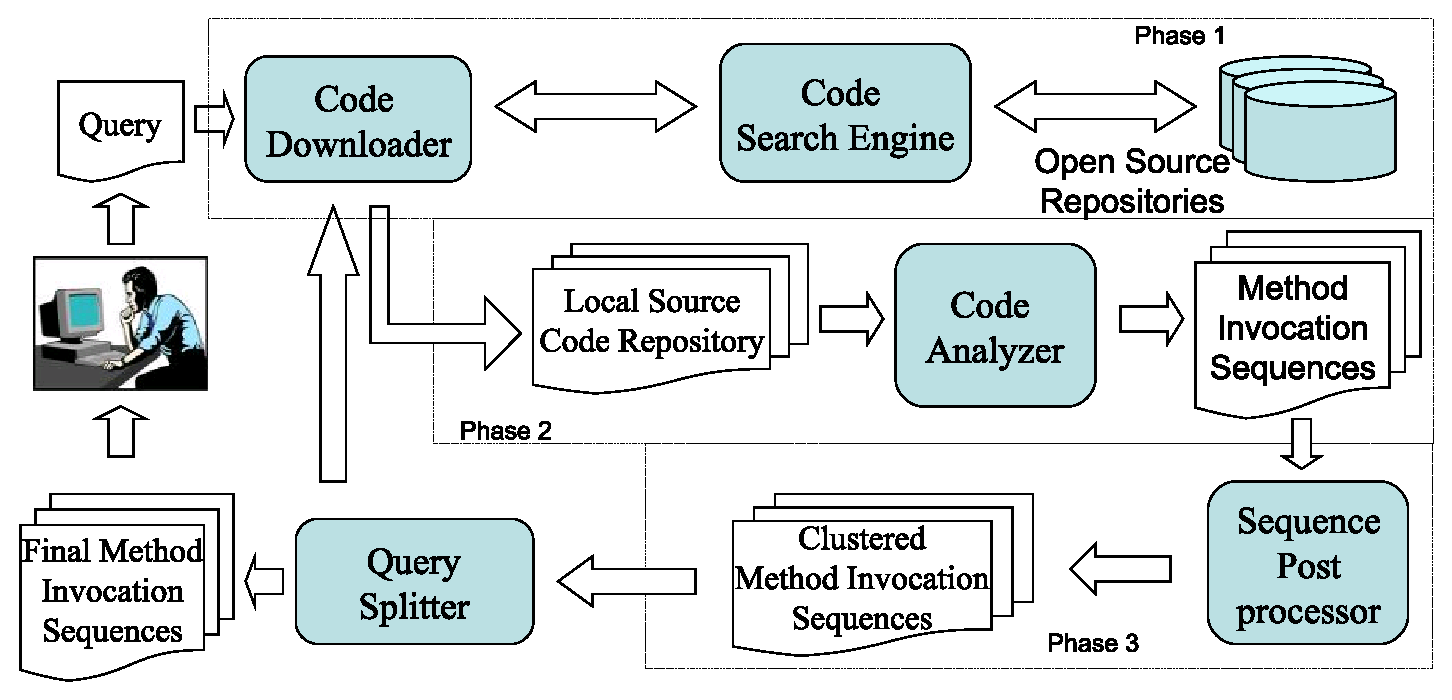
\includegraphics[scale=0.32,clip]{PARSEWeb_overview_new.eps}\vspace*{-1ex}
\caption{Overview of PARSEWeb} \label{fig:architecture}
\vspace*{-2ex}
\end{figure}
%-------------------------------------------------------------------------
\subsection{Code Search Engine}

On the web, there are a variety of
CSEs\footnote{\url{http://gonzui.sourceforge.net/links.html}}
available to assist programmers in searching for relevant code
samples like Google~\cite{GCSE} and Koders~\cite{KODERS}\Comment{,
and Krugle~\cite{KRUGLE}}. The main reason for using CSEs in our
approach is that many new frameworks or libraries emerge from day to
day and it is not practical for our own approach to maintain a
repository of all the available frameworks or libraries, and extract
results of given queries from that repository. Therefore, our
approach uses CSEs as an alternative to search in the available open
source frameworks or libraries on the web and gathers the relevant
code samples on demand. Moreover, our idea of gathering code samples
on demand makes our approach independent of any specific set of
frameworks or libraries.

In our approach, we used GCSE~\cite{GCSE} for collecting relevant code samples for the
given query, partly because GCSE provides convenient open APIs for the
third-party tools to interact with and it has been consistently
improved and maintained. However, our approach is independent of the
underlying CSE and can be extended easily to any other CSE.

%-------------------------------------------------------------------------
\subsection{Code Downloader}

The code downloader component accepts queries of the form
``\emph{Source} $\rightarrow$ \emph{Destination}'' from the
programmer and constructs a request for a CSE. The constructed
request contains both \emph{Source} and \emph{Destination} object
types. The code downloader component submits the constructed request
to CSE and downloads code samples returned by CSE to form a local
source code repository. The code samples stored in the local source
code repository are often partial and not compilable, because the
code downloader downloads only individual source files with usages
of the given \emph{Source} and \emph{Destination} object types,
instead of entire projects.
%-------------------------------------------------------------------------
\subsection{Code Analyzer}
The code analyzer component takes code samples stored in the local
source code repository as input and analyzes them to extract MISs
that can serve as solutions for the given query of the form
``\emph{Source} $\rightarrow$ \emph{Destination}''.

As code samples (i.e., source files) stored in the local source code
repository are often partial and not compilable, our approach converts
each code sample into an intermediate form. We developed the
following graph-based algorithm in the conversion process to support
method inlining and to preserve control-flow information in the
intermediate form.

Initially, the code analyzer creates an Abstract Syntax Tree (AST)
for each code sample. The code analyzer uses the created AST to
build a Directed Acyclic Graph (DAG). A node in the constructed DAG
contains a single statement and an edge represents the control flow
between the two statements. The primary advantage of DAG is that DAG
supports control-flow information through branches and joins, and
provides an effective mechanism for identifying paths between any
two nodes in the graph. The statements inside loops like
\emph{while} and \emph{for} may be executed either several times or
zero time. Considering these statements once can help generate the
MIS associated with the loop. Therefore, our approach treats the
statements inside loops like \emph{while} and \emph{for} as a group
of statements that are executed either once or not. While
constructing DAG, the code analyzer performs method inlining by
replacing the method invocations of the class under analysis with
the body of the corresponding method declarations. Our approach
cannot perform method inlining if the corresponding method
declaration is \emph{abstract}. This method inlining process helps
to identify MISs that are split among methods of the class under
analysis (shown in Section~\ref{sec:parsewebtech}). If the current
class does not contain the method declaration of a method invocation
whose receiver type is \CodeIn{this} (either explicitly or
implicitly stated at the call site), the code analyzer assumes that
this method belongs to the parent class and associates a special
context called parent context (Section~\ref{sec:parentcontext}) with
that node. When needed, the code analyzer can use this parent
context for identifying the \emph{Source} object type.

The nodes in the constructed DAG contain only those statements that
result in a transformation from one object type to another. In
particular, the statements that are included in the intermediate
form belong to one of the types described below:

\begin{Itemize}
\Item Method Invocation: Generally, a method invocation with a
non-void return type can be considered as a statement that
transforms either the receiver type \Comment{(for a non-static method
invocation)} or argument types to the return type. For example, the
method invocation \CodeIn{ReturnObj obj1 = RefObj.method(Arg1,
Arg2)} can be considered as a statement that transforms objects of
type \CodeIn{RefObj}, \CodeIn{Arg1} or \CodeIn{Arg2} to
\CodeIn{ReturnObj}.
%
\Item Constructor: As a constructor generally takes some arguments,
it can be considered as a statement that transforms objects of its
argument types to the newly created object type.
%
\Item Typecast: A typecast can be considered as a transformation
statement, because it performs an explicit transformation from one
object type to another.
\end{Itemize}

Along with identifying the preceding statement types, our
approach uses several heuristics (Section ~\ref{sec:heuristics}) to
gather additional type information for each statement and this
additional type information is associated with the corresponding
node in the graph. For example, the additional type information for
method-invocation statements include the receiver object type, the
return object type, and argument types. When any of receiver, return,
or argument types matches with the given \emph{Source} object type,
the code analyzer marks the corresponding node as a \emph{Source}
node. When the return type of any statement matches with the
required \emph{Destination} type, the code analyzer marks the
corresponding node as a \emph{Destination} node.

The code analyzer extracts a MIS from the DAG by calculating the
shortest path from a \emph{Source} node to a \emph{Destination}
node. The shortest path is sufficient as every path from
\emph{Source} to \emph{Destination} nodes contain a desired
method-invocation sequence. Once a possible sequence is identified
from the DAG, the minimization process of the code analyzer extracts
a minimal MIS from the possible sequence by eliminating the extra
method invocations that are not related to the given query. This
minimal MIS is identified by traversing the sequence in the reverse
direction from the \emph{Destination} node to the \emph{Source} node
by continuously matching the receiver type and argument types of
each statement with the return type of the preceding statements. For
example, consider a possible sequence for the query
``\CodeIn{IEditorPart} $\rightarrow$ \CodeIn{ICompilationUnit}''
(where each statement consists of the receiver type, method
name, arguments, and return type):

\begin{CodeOut}
\begin{alltt}
01:IEditorPart,getEditorInput() : IEditorInput
02:CONSTRUCTOR,Shell() : Shell
03:Shell,setText(String) : void
04:JavaUI,getWorkingCopyManager() : IWorkingCopyManager
05:IWorkingCopyManager,connect(IEditorInput) : void
06:IWorkingCopyManager,getWorkingCopy(IEditorInput)
\hspace*{0.5in}: ICompilationUnit
\end{alltt}
\end{CodeOut}

The minimization process maintains a special set called a look-up set
that initially contains only the required \emph{Destination} object.
For the given possible sequence, the process starts from Statement 6
and adds the receiver type \CodeIn{IWorkingCopyManager} and the
argument type \CodeIn{IEditorInput} to the look-up set, and removes
\CodeIn{ICompilationUnit} from the look-up set. The minimization
process retains Statement 5 in the minimal MIS as its receiver type
matches with one of the types in the look-up set. In Statement 4,
the minimization process adds \CodeIn{JavaUI} to the look-up set and
removes \CodeIn{IWorkingCopyManager}. The process ignores Statements
3 and 2 as none of its object types match with the object types in
the look-up set. The minimization process ends with Statement 1 and
generates the minimal MIS as ``1,4,5,6''. These minimal MISs are
given as input to the sequence postprocessor component
(Section~\ref{sec:miner}).
%--------------------------------------------------------------------------
\subsubsection{Type Resolution}
\label{sec:heuristics}

Heuristics play a major role in the static analysis phase of our
approach. As the downloaded code samples are often partial and not
compilable, our approach relies on these heuristics to gather
information like the receiver object type, argument types, and the
return object type of each method invocation. Our approach uses five
heuristics for identifying the receiver object type and argument
types, and uses ten heuristics for identifying the return object
type. Our heuristics are based on simple language semantics like
object types of left and right hand expressions of an assignment
statement are either same or related to each other through
inheritance. Due to space limit, we explain only two of our
major heuristics used for identifying the return type of a method
invocation.

\textbf{Type Heuristic 1:} \emph{The return type of a
method-invocation statement contained in an initialization
expression is the same as the type of the declared variable.}

Consider the code sample shown below:
\begin{CodeOut}
\begin{alltt}
QueueConnection connect; QueueSession session =
\hspace*{0.4in}connect.createQueueSession(false,int)
\end{alltt}
\end{CodeOut}

%\vspace{1ex}
The receiver type of the method
\CodeIn{createQueueSession} is the type of \CodeIn{connect}
variable. Therefore, the receiver type can be simply inferred by
looking at the declaration of the \CodeIn{connect} variable. But as
our approach mainly deals with code that is partial and not
compilable, it is difficult to get the return type of the
method-invocation  \CodeIn{createQueueSession}. The reason is the
lack of access to method declarations. However, the return type can
be inferred from the type of variable \CodeIn{session} on the left
hand side of the assignment statement. As the type of variable
\CodeIn{session} is \CodeIn{QueueSession}, we can infer that the
return type of the method-invocation \CodeIn{createQueueSession} is
\CodeIn{QueueSession}.

\textbf{Type Heuristic 2:} \emph{The return type of an outermost
method-invocation contained in a return statement is the same as the
return type of the enclosing method declaration.}

Consider code sample presented below:
\begin{CodeOut}
\begin{alltt}
\textbf{public} QueueSession test()\hspace*{0.2in}\{ ...
\hspace*{0.4in}\textbf{return} connect.createQueueSession(false,int);\}
\end{alltt}
\end{CodeOut}

In this code sample, the method-invocation statement\\
\CodeIn{createQueueSession} is a part of the return statement of the
method declaration. In this scenario, we can infer the return type of
this method-invocation from the return type of the method \CodeIn{test}.
As the method \CodeIn{test} returns \CodeIn{QueueSession}, we
can infer that the return type of the
method-invocation \CodeIn{createQueueSession} is also
\CodeIn{QueueSession}.

%-------------------------------------------------------------------------
\subsubsection{Parent Context}
\label{sec:parentcontext}
A parent context includes the parent object type, if any, and
interfaces implemented by the class in the given code sample. In some of the code
samples, we observed that the \emph{Source} object type is not
explicitly available in the code sample but is described as a
parent class. The code analyzer component handles this aspect by identifying the
parent context as possible \emph{Source} object types. Consider the
query ``\CodeIn{TextEditorAction} $\rightarrow$
\CodeIn{ITextSelection}'' and a related code sample shown below:\vspace*{-2ex}

\begin{CodeOut}
\begin{alltt}
01:public class OpenAction extends TextEditorAction \{
02:\hspace*{0.1in}public void run() \{
03:\hspace*{0.3in}ITextEditor editor = getTextEditor();
04:\hspace*{0.3in}ISelectionProvider provider =
   \hspace*{0.6in}editor.getSelectionProvider();
05:\hspace*{0.3in}ITextSelection textSelection = (ITextSelection)
   \hspace*{0.6in}provider.getSelection(); \hspace*{0.1in}\}\hspace*{0.1in}\}
\end{alltt}
\end{CodeOut}

In the preceding sample, class \CodeIn{OpenAction} declares only a
\CodeIn{run} method. Although the code sample includes a solution
for the given query, it is not explicitly available as the method
declaration of \CodeIn{getTextEditor} is not available. In this
case, we can consider that the method \CodeIn{getTextEditor} is
defined in either \CodeIn{TextEditorAction} or its parent classes.
Therefore, class \CodeIn{TextEditorAction} can be considered as
receiver type for the method \CodeIn{getTextEditor}. With this consideration, our approach can
identify that this code sample is a possible solution for the given
query.
%--------------------------------------------------------------------------
\subsection{Sequence Postprocessor}
\label{sec:miner} The sequence postprocessor component clusters similar MISs
and ranks the clustered MISs. Clustering of MISs helps to identify
distinct possible MISs and also reduces the total number of MISs.
This reduction of the number of results can help programmers quickly
identify the desired MIS for the given query. To further assist
programmers, the sequence postprocessor also sorts the clustered results.
These sorted results can help programmers identify sequences that
are more frequently used for addressing the given query.

\subsubsection{Sequence Clustering}
\label{sec:rankingCriteria}

\Comment{We observed that queries often result in similar MISs. To cluster
these similar MISs, }We next describe the heuristic used
by our approach for identifying and clustering similar MISs.
To identify similar MISs, our approach ignores the order of statements in the
extracted MISs. Our approach considers MISs with the same set of
statements and with a different order as similar.
For example, consider MISs ``2,3,4,5'' and ``2,4,3,5'' where each
number indicates a single statement associated with the node
in the constructed DAG. Our approach considers
these sequences as similar because different programmers
may write intermediate statements in different orders and these
statements may be independent from one another.

To further cluster the identified MISs, 
our approach identifies MISs with minor differences and
clusters those identified MISs. We introduce an attribute,
called \emph{cluster precision}, which defines the number of statements by
which two given MISs differ each other. This attribute is
configurable and helps the sequence postprocessor in further 
clustering the identified MISs. Our approach considers
MISs that differ by the given \emph{cluster precision} value
as similar, irrespective of the order of statements in
those MISs. For example, consider MISs ``8,9,6,7'' and ``8,6,10,7''. These two
sequences have three common statements (8,6,7) and differ by a
single statement. Our approach considers these two MISs as similar
under a \emph{cluster precision value} of one, as both the sequences
differ by only one method invocation. This heuristic is based on the
observation that different MISs in the final set of sequences often
contain overloaded forms of the same method invocation.
%-------------------------------------------------------------------------
\subsubsection{Sequence Ranking}
\label{sec:rankingCriteria}

In general, many queries result in more than one possible solution,
and not all solutions are of the same importance to the programmer.
To assist the programmer in quickly identifying the desired MISs,
our approach uses two ranking heuristics and sorts the final
set of MISs.

\textbf{Ranking Heuristic 1:} \emph{Higher the frequency
$\rightarrow$ Higher the rank}

This heuristic is based on the observation that more-used MISs might
be more likely to be used compared to less-used MISs. Therefore,
MISs with higher frequencies are given a higher preference.

\textbf{Ranking Heuristic 2:} \emph{Shorter the length $\rightarrow$
Higher the rank}

This ranking heuristic, which was originally proposed in the
Prospector~\cite{prospector:jungloid} approach, is based on the
length of the MIS. Shorter sequences are given a higher preference to
longer sequences. This heuristic is considered based on the
observation that programmers would often tend to use shorter
sequences instead of longer ones to achieve their task.

%-------------------------------------------------------------------------
\subsection{Query Splitter}
\label{sec:querysplitter}
Query splitting is an additional heuristic used by our approach to
address the problem of lack of code samples in the results of CSE.
We observed that a code sample for some of the queries is split
among different files instead of having the entire sample in the
same file. The query splitting heuristic helps to address this
problem by splitting the given query into multiple sub-queries. The
algorithm of our approach including the query splitting heuristic is
described in Algorithm ~\ref{alg:parsewebalgo}.

Initially, our approach accepts the query of the form
``\emph{Source} $\rightarrow$ \emph{Destination}'' and tries to
suggest solutions. If no possible MISs are found, our approach tries
to infer the immediate alternate destinations (\emph{AltDest}) by
constructing a new query that includes only the \emph{Destination}
object type. A query with just the \emph{Destination} object
type provides different possible MISs, referred as
\emph{DestOnlyMISs}, that result in the object of the
\emph{Destination} type. In these \emph{DestOnlyMISs}, the
\emph{Source} can be of any object type. Our approach infers the
\emph{AltDestSet} by identifying the receiver type and argument
types in the last method invocation (\emph{lastMI}) of each MIS in
the \emph{DestOnlyMISs} set. The primitive types, such as
\CodeIn{int}, are ignored while identifying the \emph{AltDest}. For
each of the \emph{AltDest}, new MISs are generated by constructing
queries of the form ``\emph{Source} $\rightarrow$ \emph{AltDest}''.
The \emph{lastMI} of the earlier sequence is appended to the new set
of sequences to generate a complete MIS. In case our approach
including the query splitting is not able to suggest any MISs, we
simply return the \emph{DestOnlyMISs}.

\begin{algorithm}[t]
\begin{CodeOut}
\SetLine
\KwIn{Source and Destination object types}
\KwOut{Method-Invocation Sequences}
Extract $MISs$ for the Query ``Source$\rightarrow$Destination''\;
\If{$MISs$ are not empty}{\Return MISs\;}
//Query Splitting\\
Extract $DestOnlyMISs$ for the Query ``Destination''\;
\For{$MIS$ in $DestOnlyMISs$}{
$lastMI$ = $MIS$.lastMethodInvocation()\;
$AltDestSet$ = $ReceiverType$ and $ArgTypes$ of $lastMI$\;
Intialize $FinalMISs$\;
\For{$AltDest$ in $AltDestSet$}{
Extract $AltMIS$ for the Query ``Source$\rightarrow$AltDest''\;
Append $lastMI$ to $AltMIS$\;
Add $AltMIS$ to $FinalMISs$\;
}}
\If{$FinalMISs$ are not empty}{
\Return $FinalMISs$
}\Else{\Return $DestOnlyMISs$\;}
\end{CodeOut}
\caption{Pseudocode of the PARSEWeb algorithm with the query
splitting heuristic} \label{alg:parsewebalgo}
\end{algorithm}

%-------------------------------------------------------------------------
\section{Implementation}
\label{sec:implementation}
%--------------------------------------------------------------------
\begin{figure*}[t]
\centering
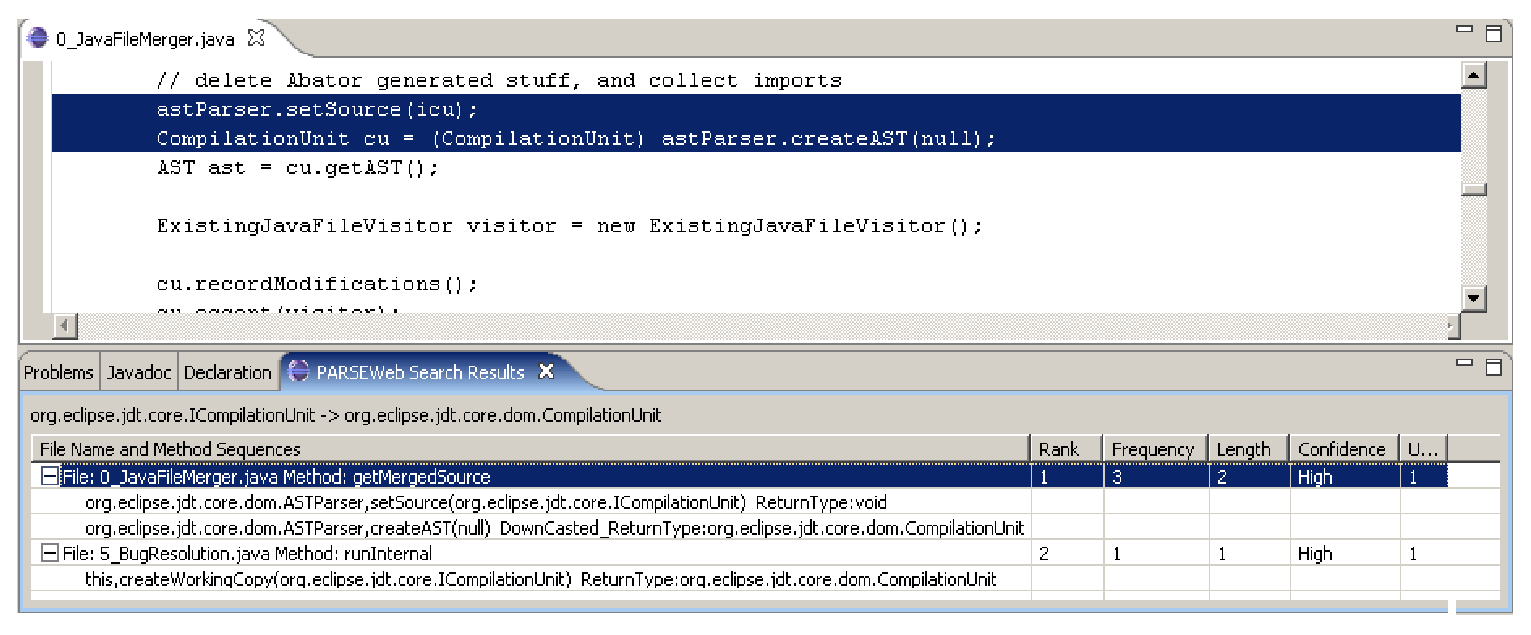
\includegraphics[scale=0.50,clip]{plugin_image1.eps}\vspace*{-2ex}
\caption{A snapshot of PARSEWeb plugin interface} \label{fig:plugin}
\vspace*{-2ex}
\end{figure*}
%--------------------------------------------------------------------
We used Google Code Search Engine (GCSE)~\cite{GCSE} as an
underlying CSE for the code downloader component. To improve
performance, the code downloader uses the multi-threading feature of
the Java programming language, and\Comment { to enable parallel
download of multiple source files. As the source files returned by
GCSE~\cite{GCSE} are in the HTML format, the code downloader}
invokes a post processor written in the Perl language to transform
the source files returned by GCSE from HTML to Java. Eclipse JDT
Compiler~\cite{java:eclipse} is used for building ASTs from Java
files.\Comment{We used a Directed Acyclic Graph (DAG) for
representing the intermediate form, because DAG provides an easy
mechanism for traversing from the \emph{Destination} object type to
the \emph{Source} object type as required by our approach.} We used
Dijkstra's shortest path algorithm from the Jung~\cite{Jung} library
\Comment{\Fix{May need to cite an algorithm textbook}} to gather the
required path from \emph{Source} to \emph{Destination} object types.

We developed an Eclipse plugin, called PARSEWeb\footnote{Available at
\url{http://ase.csc.ncsu.edu/parseweb/}}, that integrates all described aspects
of our approach. PARSEWeb displays the suggested MISs for the given
query in a tree-structured tabular form. A snapshot of our PARSEWeb
output is shown in Figure~\ref{fig:plugin}. Each MIS is associated
with additional information like rank, frequency, and length. \Comment{As
described in Algorithm~\ref{alg:parsewebalgo}, PARSEWeb
may return the results of the query with only the \emph{Destination}
object type. This case can happen if PARSEWeb fails to identify the
exact code samples. In such cases, the \emph{Confidence} information
shown in the snapshot is set to ``Low''.}Programmers can browse the
relevant code sample of the suggested MIS by double clicking on the
corresponding entry.

The current implementation of PARSEWeb shows only the first ten MISs
that can serve as a solution for the given query. Furthermore, the
query splitter is configured to iterate all three main phases
for only the first five elements in \emph{DestOnlyMISs} (shown in
Algorithm~\ref{alg:parsewebalgo}). However, both these parameters are
configurable through the property file.

%-------------------------------------------------------------------------
\section{Evaluation}
\label{sec:evaluation}

We conducted four different evaluations on PARSEWeb to show that
PARSEWeb is effective in solving programmers' queries. In the
first evaluation, we showed that PARSEWeb is able to solve
programming problems posted in developer forums of existing
libraries. In the second evaluation, we showed that
PARSEWeb-suggested solutions are available in \realprojects{}. We
also analyzed the PARSEWeb results with the results of two other
related tools:
Prospector\footnote{\url{http://snobol.cs.berkeley.edu/prospector/}}~\cite{prospector:jungloid}
and
Strathcona\footnote{\url{http://strathcona.cpsc.ucalgary.ca/}}~\cite{strathcona:se}.
Prospector tries to solve the queries related to a specific set of
frameworks or libraries by using API signatures. Strathcona tries to
suggest similar code examples stored in an example repository by
matching the context of the code under development with the samples
stored in the example repository. In the third evaluation, we
compared PARSEWeb with Prospector. We showed that PARSEWeb performs
better than Prospector. Moreover, PARSEWeb is not limited to the
queries of any specific set of frameworks or libraries as Prospector
is. In the fourth evaluation, we showed the significance of different techniques used
in PARSEWeb.

%-------------------------------------------------------------------------
\subsection{Programming Problems}
\label{sec:subexperiments}

The purpose of this evaluation is to show that PARSEWeb is not
limited to the queries of any specific set of frameworks or
libraries. We collected two programming problems that were posted
by developers in forums of existing open source frameworks or
libraries and checked whether PARSEWeb is able to suggest solutions
for those problems; existing tools such as Prospector and Strathcona
cannot address these problems because the queries for these problems
fall out of the scope of these two tools: J2SE, Eclipse, and Eclipse
GEF (Graphical Editing Framework). The results indicate that PARSEWeb is able to solve
these real programming problems.

%-------------------------------------------------------------------------
\subsubsection{Jakarta BCEL User Forum}

The Byte Code Engineering Library (BCEL) provides the ability to
analyze, create, and manipulate Java bytecode files.\Comment{BCEL is
already being used successfully in several projects such as
compilers, optimizers, and code generators.} We collected the
programming problem ``How to disassemble Java byte code'' posted in
the BCEL forum~\cite{BCELForum}. The programming problem describes
that the programmer is using the BCEL library and has Java byte code
under analysis. In the BCEL library, Java byte code is represented
through the \CodeIn{Code} class. The programmer wants to obtain a
Java assembler command list, which is represented in the form of
instructions in the BCEL library. Therefore, we identified the
relevant query for the given problem description as ``\CodeIn{Code}
$\rightarrow$ \CodeIn{Instruction}''. PARSEWeb suggested a solution
for the query as shown below:

\begin{CodeOut}
\begin{alltt}
01:FileName:2\_RepMIStubGenerator.java MethodName:
\hspace*{0.2in}isWriteMethod Rank:1 NumberOfOccurrences:1
02:Code,getCode() ReturnType:\#UNKNOWN\#
03:CONSTRUCTOR,InstructionList(\#UNKNOWN\#)
\hspace*{0.2in}ReturnType:InstructionList
04:InstructionList,getInstructions() 
\hspace*{0.2in}ReturnType:Instruction
\end{alltt}
\end{CodeOut}

The suggested solution is the same as the response posted in the forum. The programmer
can refer to a related code sample by browsing the \CodeIn{isWriteMethod} method
in the file \CodeIn{2\_RepMIStubGenerator.java}. 
The original code sample collected from the
preceding method is shown below:

\begin{CodeOut}
\begin{alltt}
Code code;
InstructionList il = new InstructionList(code.getCode());
Instruction[] ins = il.getInstructions();
\end{alltt}
\end{CodeOut}

In the code sample suggested by PARSEWeb, the return type of
\CodeIn{getCode} method is described as \CodeIn{UNKNOWN}. The keyword
\CodeIn{UNKNOWN} denotes that the PARSEWeb is not able to infer the
return type through its heuristics, because the return type of
\CodeIn{getCode} method is not explicitly specified in the code
sample. However, PARSEWeb still correctly suggested to pass the
return type directly to the constructor of \CodeIn{InstructionList}.
%-------------------------------------------------------------------------

\Comment{\subsubsection{Java Media Framework forum}

The Java Media Framework API (JMF) enables audio, video, and other
time-based media to be added to applications and applets built on
Java technology. We collected the programming problem ``Get the Data
from a DataSource'' posted by a JMF developer from the JMF
forum~\cite{JMFForum}. The main objective of the problem was to get
raw data from an object of type \CodeIn{Processor}. We transformed
the problem into the query ``\CodeIn{Processor $\rightarrow$}
\CodeIn{PushBufferStream}'' by using the description given in the
problem. We specified the \emph{Destination} as
\CodeIn{PushBufferStream}, because raw data can be obtained from a
\CodeIn{BufferStream} object. We used PARSEWeb to solve the problem
and posted the solution in the forum to get developers feedback. The
solution suggested by PARSEWeb is shown below.  In the output of
PARSEWeb, the keyword ``DownCasted\_ReturnType'' indicates that an
explicit typecast has to be performed.

\begin{CodeOut}
\begin{alltt}
01: FileName:0\_CamDriver.java MethodName:initImageFetcher
02: \hspace*{0.2in}Rank:1 NumberOfOccurrences:1 Path:1 2
03: \hspace*{0.1in}javax.media.Processor,getDataOutput()
04: \hspace*{0.2in}DownCasted\_ReturnType:
05: \hspace*{0.2in}javax.media.protocol.PushBufferDataSource
06: \hspace*{0.1in}javax.media.protocol.PushBufferDataSource,getStreams()
07: \hspace*{0.2in}ReturnType:javax.media.protocol.PushBufferStream
\end{alltt}
\end{CodeOut}}
%-------------------------------------------------------------------------
\subsubsection{Dev2Dev Newsgroups}

We applied PARSEWeb on another problem ``how to connect db by
sessionBean'' posted in the Dev2Dev Newsgroups~\cite{BEAForum}. We
transformed the question into the query ``\CodeIn{InitialContext
$\rightarrow$ Connection}'' and used PARSEWeb to obtain the
solution. PARSEWeb suggested the following solution, which is the
same as the one described in the forum.

\begin{CodeOut}
\begin{alltt}
01:FileName:3\_AddrBean.java MethodName:getNextUniqueKey
\hspace*{0.2in}Rank:1 NumberOfOccurrences:34
02:InitialContext,lookup(String) ReturnType:DataSource
03:DataSource,getConnection() ReturnType:Connection
\end{alltt}
\end{CodeOut}

%-------------------------------------------------------------------------
\subsection{Real Project}

\Comment{ \setlength{\tabcolsep}{1pt}
\begin{table}[t]
%\begin{alltt}
\begin{CodeOut}
\begin{center}
\centering \caption {\label{table:codesamples} Suggested Code
Samples}
\begin {tabular} {|l|l|}
\hline \textbf{Original Code}&\textbf{PARSEWeb}\\
\hline
public void init(IPageSite &FileName:0\_JDEv...Editor.java \\
\hspace*{0.2in}pageSite)\{...&\hspace*{0.2in}MethodName:init Rank:1 \\
IActionBars bars = &NumberOfOccurrences:7 \\
\hspace*{0.2in}pageSite.getActionBars();&org.eclipse.ui.part.IPageSite\\
&,getActionBars()\\
\}&RetType:org.eclipse.ui.IActionBars\\
\hline \textbf{Prospector}&\textbf{Strathcona}\\
\hline org.eclipse.ui.part.IPageSite ips;&IActionBars actionBars =\\
org.eclipse.ui.IActionBars iab = &pageSite.getActionBars();\\
\hspace*{0.2in}ips.getActionBars();&\\
\hline
\end{tabular}
\end{center}
\end{CodeOut}
%\end{alltt}
\end{table}
}

We next show that PARSEWeb-suggested MISs exist in \realprojects{},
and compare the results with those of two related tools: Prospector
and Strathcona. As described by Bajracharya et
al.~\cite{sourcerer:baj}, there is still a need (but lack) of a
benchmark for open source code search that can be used by similar
tools for comparing their results. In our evaluation, we used an
open source project \emph{Logic}~\cite{Logic} as a subject project.
The \emph{Logic} project was developed based on Eclipse Graphical
Editing Framework (GEF). The reason for choosing \emph{Logic} for
evaluation is that \emph{Logic} is one of the standard example
projects delivered with the Eclipse GEF framework.

To be fair in evaluation, we chose all queries from the largest
source file (``LogicEditor.java'') of the subject project. 
By choosing the largest file, we can also find many
queries that can be used to evaluate all three tools. Within the
source file, we picked the first ten available queries of the form
``\emph{Source} $\rightarrow$ \emph{Destination}'' from the
beginning of the class, and used all three tools to suggest
solutions for each query. The query selection process is based on
two criteria: a new object type is instantiated from one of the
known object types and the selected query is the maximal possible
query, which we shall explain next through the code sample
extracted from the source file used in the evaluation:

\begin{CodeOut}
\begin{alltt}
01:public void createControl(Composite parent)\{
02:\hspace*{0.1in}PageBook pageBook = new PageBook(parent, SWT.NONE);
03:\hspace*{0.1in}Control outline = getViewer().createControl(pageBook);
04:\hspace*{0.1in}Canvas overview = new Canvas(pageBook, SWT.NONE);
05:\hspace*{0.1in}pageBook.showPage(outline);
06:\hspace*{0.1in}configureOutlineViewer();
07:\hspace*{0.1in}hookOutlineViewer();
08:\hspace*{0.1in}initializeOutlineViewer();\}
\end{alltt}
\end{CodeOut}

The possible queries that can be extracted from this code sample are
``Composite $\rightarrow$ PageBook'', ``Composite $\rightarrow$
Control'', and ``Composite $\rightarrow$ Canvas''. However, the
maximal possible query among these three queries is ``Composite
$\rightarrow$ Canvas'', as this query subsumes the other two
queries. We consider a task as successful only when the suggested
code sample is the same as the code snippet in the corresponding
subject project. As our approach tries to suggest solutions from
available open source repositories, which may include the subject
project under consideration, we excluded the results of PARSEWeb
that are suggested from the subject project under consideration.

As both PARSEWeb and Prospector accept the query of the preceding
form, we gave constructed queries directly as input. Strathcona
compares the context of code given as input and  suggests relevant
code samples. Therefore, for each evaluation, we built separate
driver code that can convey the context of the query. In the driver
code, we declared two local variables with the \emph{Source} and
\emph{Destination} object types, respectively.

\setlength{\tabcolsep}{1pt}
\begin{table}[t]
\begin{SmallOut}
\begin{CodeOut}
\begin{center}
\centering \caption {\label{tab:realprojevaluation} Evaluation results of programming tasks from
the Logic Project}
\begin {tabular} {|l|l|c|c|c|c|c|c|c|}
\hline
\multicolumn{2}{|c|}{Query}&\multicolumn{2}{|c|}{PARSE}&\multicolumn{2}{|c|}{PROS}&\multicolumn{2}{|c|}{Strath}&GCSE\\
\cline{1-8}
Source&Destination&No&Ra&No&Ra&No&Ra&\\
\hline
\hline IPageSite&IActionBars&1&1&3&1&10&7&1\\
\hline ActionRegistry&IAction&3&1&4&1&10&3&2\\
\hline ActionRegistry&ContextMenu&Nil&Nil&2&2&10&3&NA\\
                &Provider&&&&&&&\\
\hline IPageSite&ISelection&1&1&12&1&10&Nil&5\\
             &Provider&&&&&&&\\
\hline IPageSite&IToolBar&2&1&12&1&10&6&9\\
              &Manager&&&&&&&\\
\hline String&ImageDescriptor&10&6&12&Nil&10&Nil&28\\
\hline Composite&Control&10&2&12&Nil&10&Nil&72\\
\hline Composite&Canvas&10&5&12&Nil&10&Nil&28\\
\hline GraphicalViewer&Scrollable&2&1&12&8&10&7&2\\
              Thumbnail&&&&&&&&\\
\hline GraphicalViewer&IFigure&1&Nil&12&Nil&10&Nil&NA\\
\hline
\end{tabular}
\CodeIn{PARSE: PARSEWeb, PROS: Prospector, Strath: Strathcona
No: Number, Ra: Rank}
\end{center}
\end{CodeOut}
\end{SmallOut}
\vspace*{-6ex}
\end{table}
We used PARSEWeb, Prospector, and Strathcona to suggest solutions
for each query. The results of our evaluation are shown in
Table~\ref{tab:realprojevaluation}. \Comment{Column ``Query'' shows the query
given as input. Columns ``Source'' and ``Destination'' show the
\emph{Source} and \emph{Destination} object types, respectively.}
In Columns ``PARSE'', ``PROS'', and ``Strath'',
Sub-columns ``No'' and ``Ra'' show the
number of results returned by each tool, and rank of the suggested
solution that matches with the original source code of the subject
project from which the query is constructed. The maximum number of
results returned by PARSEWeb, Prospector, and Strathcona are $10$, $12$,
and $10$, respectively. The last column ``GCSE'' shows the index of the
source file that contained the solution among the results by GCSE.
This index information is extracted by identifying the first source
file in which the resultant MIS is found.
We found that both PARSEWeb and Prospector performed better than
Strathcona. Between PARSEWeb and Prospector, PARSEWeb performed
better than Prospector.\Comment{ We presented the original source
code and the solutions suggested by each tool for the first case in
Table~\ref{table:codesamples}. It is easy to identify that the
solutions suggested by each tool are the same as original source
code.} We next discuss the results of each tool individually.

From the results, we observed that PARSEWeb suggested solutions for all queries except for two.
The reason behind the better performance of PARSEWeb
is that PARSEWeb suggests solutions from reusable code samples.
We inspected queries for which PARSEWeb could not suggest any solution and found the reason
is a limitation of our approach in analyzing partial code samples.
We elaborate this limitation in Section~\ref{sec:discussion}.

Prospector tries to solve the given query using API signatures.
Therefore, it can often find some feasible solution for a given
query, as it can find a path from the given \emph{Source} to
\emph{Destination}. One reason for not getting complete results with
Prospector in our evaluation could be that Prospector shows only
first twelve results of the given query. Due to this limitation, the
required solution might not have shown in the suggested set of
solutions. Prospector solves the queries through API signatures and
has no knowledge of which MISs are often used compared to other
MISs that can also serve as a solution for the given query. PARSEWeb
performs better in this scenario because PARSEWeb tries to suggest
solutions from reusable code samples and is able to identify MISs
that are often used for solving a given query. For example, for
query ``\CodeIn{Composite} $\rightarrow$ \CodeIn{Canvas}'', the
solution is through an additional class called \CodeIn{PageBook}. Although
this solution is often used, Prospector is not able to identify the
solution as it can be a less favorable solution from the API signature point-of-view.

We suspect that the reason for not getting good results with
Strathcona is that Strathcona cannot effectively address the queries
of the form ``\emph{Source} $\rightarrow$ \emph{Destination}''. We
observed that Strathcona generates relevant solutions when the exact
API is included in the search context.
But our described problem is to identify that API, as
the programmer has no knowledge of which API has to be used for
solving the query. Moreover, we found that many code samples
returned by Strathcona contain both \emph{Source} and
\emph{Destination} object types in either \CodeIn{import} statements
or in different method declarations. Therefore, those code samples
cannot address our query as no MIS can be derived to lead from
\emph{Source} to \emph{Destination} object types.

The results shown in Column ``GCSE'' indicate the problems that may
be faced by programmers in using CSEs directly. For
example, to find the solution for the seventh task, the programmer
has to check 72 files in the results of GCSE.
%-------------------------------------------------------------------------
%-------------------------------------------------------------------------
\subsection{Comparison of PARSEWeb and \\Prospector}
\label{sec:parseweb_pros}

We next present the evaluation results of PARSEWeb and
Prospector\footnote{We chose only Prospector for detailed comparison
because another related tool XSnippet~\cite{xsnippet:saha} was not
available and Strathcona did not perform well in addressing the
described problem based on the previous evaluation.} for 12 specific
programming tasks. These tasks are based on Eclipse plugin examples
from the \emph{Java Developer's Guide to Eclipse}~\cite{java:eclipse} and are the same as the first 12 tasks
used by Sahavechaphan and Claypool~\cite{xsnippet:saha} in
evaluating their XSnippet tool. We have not chosen the remaining 5
tasks used in evaluating the XSnippet tool as they are the same as
some previous tasks, but differ in the code context where the tasks
are executed. As neither PARSEWeb nor Prospector considers the code
context, these 5 tasks are redundant to use in our evaluation.

The primary reason for selecting these tasks are that their
characteristics include different Java programming aspects like
object instantiation via a constructor, a static method, and a
non-static method from a parent class. These tasks also require
downcasts and have reasonable difficulty levels. For each task, all
necessary Java source files and Jar files are provided and code for
getting the \emph{Destination} object from the \emph{Source} object
is left incomplete. We used open source projects such as
\CodeIn{org.eclipse.jdt.ui}, and examples from Eclipse corner
articles\footnote{\url{http://www.eclipse.org/articles/}} for
creating the necessary environment. We used PARSEWeb and Prospector
to suggest solutions for each query. A task is considered as
successful if the final code can be compiled and executed, and the
required functionality is enabled with at least one suggested
solution. The task is also considered as successful if the suggested
solution acts as a starting point and the final code could be
compiled with some additional code. Prospector can generate
compilable code for its suggested solutions, but the current
implementation of PARSEWeb suggests only the frequent MISs and code
samples, but cannot directly generate compilable code. Therefore, we
manually transformed the suggested sequences into appropriate code
snippets.
%--------------------------------------------------------------------------
\setlength{\tabcolsep}{3pt}
\begin{table}[t]
\begin{SmallOut}
\begin{CodeOut}
\begin{center}
\centering \caption {\label{table:evaluation} Evaluation results of
programming tasks previously used in evaluating the XSnippet
tool}
\begin {tabular} {|l|l|c|c|}
\hline \multicolumn{2}{|c|}{Query}&PARSE&PROS\\
\cline{1-2}
Source&Destination&&\\
\hline
\hline ISelection&ICompilationUnit&Yes&No\\
\hline IStructuredSelection&ICompilationUnit&Yes&Yes\\
\hline ElementChangedEvent&ICompilationUnit&Yes&Yes\\
\hline IEditorPart&ICompilationUnit&Yes&Yes\\
\hline IEditorPart&IEditorInput&Yes&Yes\\
\hline ViewPart&ISelectionService&Yes&Yes\\
\hline TextEditorAction&ITextEditor&Yes&No\\
\hline TextEditorAction&ITextSelection&Yes&No\\
\hline ITextEditor&ITextSelection&Yes&Yes\\
\hline AbstractDecorated&ProjectViewer&No&No\\
             TextEditor&&&\\
\hline TextEditor&IDocument&Yes&No\\
\hline TextEditor&ITextSelection&Yes&Yes\\
\hline
\end{tabular}
\end{center}
\end{CodeOut}
\end{SmallOut}
\vspace*{-6ex}
\end{table}

The results of our evaluation for the $12$ programming
tasks are shown in Table~\ref{table:evaluation}. PARSEWeb is not able to suggest
solution for only one query, whereas Prospector failed to suggest
solutions for five queries. This result demonstrates the strength of
PARSEWeb as it suggests solutions from reusable code samples
gathered from publicly available source code repositories. A summary
of percentage of tasks successfully completed by each tool along
with the results collected from the XSnippet~\cite{xsnippet:saha}
approach is shown in Figure~\ref{fig:resultschart}. The x axis
shows different tools and the y axis shows the percentage of tasks
successfully completed by each tool. The ``XSnippet1'' and
``XSnippet2'' entries show two XSnippet query-type techniques:
\emph{Type-Based Instantiation Query} ($IQ_{T}$) and
\emph{Generalized Instantiation Query} ($IQ_{G}$), respectively.
PARSEWeb performed better than Prospector and XSnippet's $IQ_{T}$
query type. The results of PARSEWeb are at par with XSnippet's
$IQ_{G}$ query type. However, the $IQ_{G}$ query type of XSnippet
cannot effectively address the issue targeted by PARSEWeb as
this query type simply returns the set of all code samples contained in the
sample repository that instantiate the given \emph{Destination}
object type, irrespective of the \emph{Source} object type. Moreover, XSnippet
is also limited to the queries of a specific set of frameworks or
libraries.
%-------------------------------------------------------------------------
\subsection{Significance of PARSEWeb Techniques}
\label{sec:parsewebtech}
\setlength{\tabcolsep}{1pt}
\begin{table}[t]
\begin{SmallOut}
\begin{CodeOut}
\begin{center}
\centering \caption {\label{tab:internaltech} Evaluation results
 of PARSEWeb internal techniques}
\begin {tabular} {|l|l|c|c|c|c|}
\hline
\multicolumn{2}{|c|}{Query}&Simple&Method&Post&Query\\
\cline{1-2}
Source&Destination&&Inline&Process&Split\\
\hline
\hline TableViewer&TableColumn&21&23&2&2\\
\hline IWorkbench&IEditorPart&13&17&8&8\\
\hline IWorkBench&IStructured&5&6&1&1\\
             Page&Selection&&&&\\
\hline Composite&Control&26&29&24&24\\
\hline IEditorSite&ISelectionService&Nil&Nil&Nil&2\\
\hline
\end{tabular}
\end{center}
\end{CodeOut}
\end{SmallOut}
\vspace*{-4ex}
\end{table}

We next show the significance and impact of different techniques
used in PARSEWeb. We picked some of the queries in preceding
evaluations and analyzed different techniques of our approach. The
results of our analysis are shown in Table ~\ref{tab:internaltech}.
The table shows the number of identified MISs after applying respective
techniques. \Comment{Column ``Query'' shows the query given as input. Columns
``Simple'', ``Method Inlining'', ``Miner'', and ``Query Splitter''
show the number of results generated after applying respective
techniques.} As shown in the results, the method inlining technique
increases the possible number of sequences, whereas the sequence
postprocessing technique helps in reducing the number of sequences
by clustering similar sequences. The query splitting heuristic helps
address the lack of code samples by splitting the query into
different sub-queries.
\begin{figure}[t]
\centering
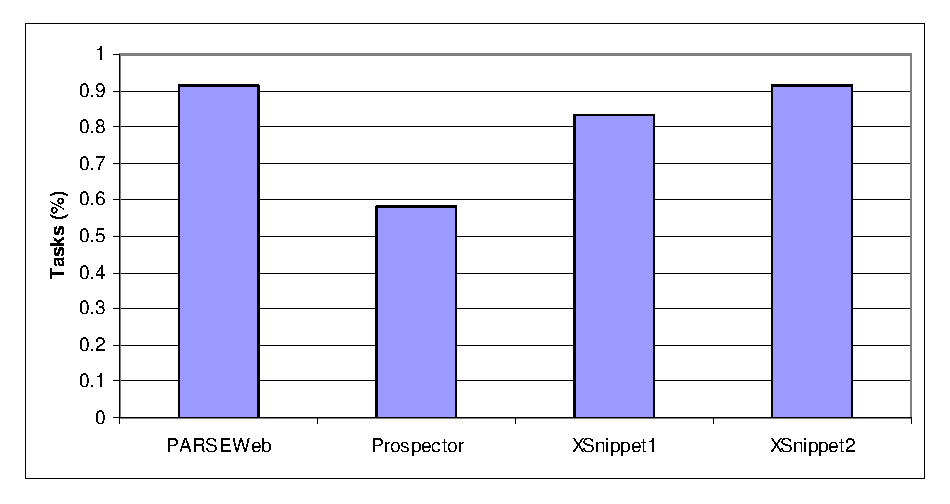
\includegraphics[scale=0.5,clip]{ComparisonResults.eps}\vspace*{-2ex}
\caption{Percentage of tasks successfully completed by PARSEWeb,
Prospector, and XSnippet} \label{fig:resultschart} \vspace*{-3ex}
\end{figure}
%-------------------------------------------------------------------------
\subsection{Summary}

The primary advantage of PARSEWeb compared to other related tools is
that PARSEWeb is not limited to the queries of any specific set of
frameworks or libraries. We showed this advantage in the first part
of our evaluation. Although Prospector solves the queries of a
specific set of frameworks or libraries from the API signatures, we
showed that the results of PARSEWeb are better than the results of
Prospector. The reason is that Prospector has no knowledge of which
MISs are often used compared to other
possible sets of sequences. This lack of information often results in
irrelevant solutions. Although both PARSEWeb and Strathcona suggest
solutions from code samples, the results of PARSEWeb are better than
Strathcona because the number of available code samples are limited
for Strathcona. Moreover, PARSEWeb has many specialized heuristics
compared to Strathcona for helping identify the required MIS. We
also showed that GCSE alone cannot handle the queries of the form
``\emph{Source} $\rightarrow$ \emph{Destination}'', and showed the
significance and impact of different techniques in PARSEWeb.


%-----------------------------------------------------------------------------
\section{Discussion and Future work}
\label{sec:discussion} In our current implementation, PARSEWeb
interacts with Google Code Search Engine~\cite{GCSE} for gathering
relevant code samples. Therefore, our current results are dependent
on code samples returned by GCSE. We observed that PARSEWeb is not
able to suggest solutions for some of the queries due to lack of
relevant code samples in the results returned by GCSE. We found this
limitation when we evaluated with open source projects
\emph{ASTView}\footnote{\url{http://www.eclipse.org/jdt/ui/astview/index.php}}
and
\emph{Flow4j}\footnote{\url{http://sourceforge.net/projects/flow4jeclipse}},
where Prospector or Strathcona also could not work well. We
alleviated this problem to a certain extent through the query
splitting heuristic. To address the problem further, We plan to
extend our tool to collect code samples from other CSEs such as
Koders~\cite{KODERS}\Comment{ and Krugle~\cite{KRUGLE}}, and analyze
the results to compare different CSEs. We expect that the addition
of new source code repositories to CSEs can also help in alleviating
the current problem.

As our approach deals with code samples that are often partial and not
compilable, there are a few limitations in inferring the information
related to method invocations. We explain the limitation of our
approach through the code sample shown below:

\vspace*{-1ex}
\begin{CodeOut}
\begin{alltt}
QueueConnectionFactory factory = jndiContext.lookup("t");
QueueSession session = factory.createQueueConnection()
\hspace*{0.2in}.createQueueSession(false,Session.AUTOACKNOWLEDGE);
\end{alltt}
\end{CodeOut}
\vspace*{-1ex}

In the second expression of this code sample, our heuristics cannot
infer the receiver type of the \CodeIn{createQueueSession} method
and the return type of the \CodeIn{createQueueConnection} method.
The reason is lack of information regarding the intermediate object
returned by the \CodeIn{createQueueConnection} method. If this intermediate
object is either \emph{Source} or \emph{Destination} of the given
query, we cannot suggest this MIS as a solution. 
Because of this limitation, our approach could not suggest
solutions to some of the queries used in evaluation.

Another issue addressed by our approach is the processing of data
returned by GCSE~\cite{GCSE}. A query such as
``\CodeIn{Enumeration} $\rightarrow$ \CodeIn{Iterator}'' results in
nearly $22,000$ entries. To avoid high runtime costs of downloading and analyzing
the code samples, PARSEWeb downloads only a fixed number of
samples, say $N$. This parameter $N$ is made as a configurable
parameter. The default value of $N$ is set to $200$, which is derived
from our experiments and identified to be large enough to make sure
that only little useful information is lost during downloading.

The current implementation of PARSEWeb can also accept queries
including only the \emph{Destination} object type. Such queries can
help programmers if they are not aware of the \emph{Source} object
type. However, the number of results returned by PARSEWeb for such
queries are often large ($10$ to $50$) due to lack of knowledge of
the \emph{Source} object type. Therefore, to reduce the number of
results and help programmers in quickly identifying the desired MIS,
we plan to extend our tool to infer the \emph{Source} object type
from the given code context. We also plan to extend our tool to
automatically generate compilable source code from the selected MIS.
 \Comment{Our current implementation cannot effectively handle
sequences that involve primitive data types as connector objects
between the given \emph{Source} and \emph{Destination} object types.
We plan to extend our approach to match on variable names also along
with data types to effectively handle primitive data types.}


%-------------------------------------------------------------------------
\section{Conclusion}
\label{sec:conclusion}

We have developed PARSEWeb, an approach for addressing problems
faced by programmers in reusing existing frameworks or libraries.
Our approach accepts queries of the form ``\emph{Source}
$\rightarrow$ \emph{Destination}'' as input and suggests
method-invocation sequences that can take the \emph{Source} object
type as input and result in the \emph{Destination} object type. Our
approach collects the relevant code samples, which include
\emph{Source} and \emph{Destination} object types, on demand from CSE.
This new idea of collecting sources on demand makes our approach 
independent of any specific set of
frameworks or libraries. Our approach includes several heuristics to
deal with partial and non-compilable code downloaded from CSE. Our 
query splitting heuristic addresses the problem of lack of
code samples by splitting the given query into multiple sub-queries.
We have conducted four different evaluations on our
approach. Through these evaluations, we showed that our approach is effective
in addressing the issues faced by programmers and performed
better than existing related tools.

\section*{Acknowledgments}

This work is supported in part by NSF grant CNS-0720641.

%-------------------------------------------------------------------------
%\end{document}  % This is where a 'short' article might terminate
%
% The following two commands are all you need in the
% initial runs of your .tex file to
% produce the bibliography for the citations in your paper.
\bibliographystyle{abbrv}
\begin{thebibliography}{10}

\bibitem{java:eclipse}
J.~Anjou, S.~Fairbrother, D.~Kehn, J.~Kellerman, and P.~McCarthy.
\newblock {\em The {J}ava Developer's Guide to Eclipse}.
\newblock Addison-Wesley Professional, 2004.

\bibitem{sourcerer:baj}
S.~Bajracharya, T.~Ngo, E.~Linstead, Y.~Dou, P.~Rigor, P.~Baldi, and C.~Lopes.
\newblock {S}ourcerer: A search engine for open source code supporting
  structure-based search.
\newblock In {\em Proc. of OOPSLA Companion}, 2006.

\bibitem{BCELForum}
{J}akarta {BCEL} user forum, 2001.
\newblock
  \url{http://mail-archives.apache.org/mod_mbox/jakarta-bcel-user/200609.mbox/%
thread}.

\bibitem{BEAForum}
Dev2{D}ev {N}ewsgroups by developers, for developers, 2006.
\newblock
  \url{http://forums.bea.com/bea/message.jspa?messageID=202265042&tstart=0}.

\bibitem{GCSE}
Google {C}ode {S}earch {E}ngine, 2006.
\newblock \url{http://www.google.com/codesearch}.

\bibitem{strathcona:se}
R.~Holmes and G.~Murphy.
\newblock Using structural context to recommend source code examples.
\newblock In {\em Proc. of ICSE}, pages 117--125, 2005.

\bibitem{Jung}
Jung the {J}ava {U}niversal {N}etwork/{G}raph {F}ramework, 2005.
\newblock \url{http://jung.sourceforge.net/}.

\bibitem{KODERS}
The {K}oders source code search engine, 2005.
\newblock \url{http://www.koders.com}.

\bibitem{document:leth}
T.~Lethbridge, J.~Singer, and A.~Forward.
\newblock How software engineers use documentation: The state of the practice.
\newblock In {\em IEEE Software}, pages 35--39, 2003.

\bibitem{Logic}
{L}ogic {P}roject based on {E}clipse {G}{E}{F}, 2006.
\newblock
  \url{http://www.eclipse.org/downloads/download.php?file=/tools/gef/downloads%
/drops/R-3.2.1-&200609211617/GEF-examples-3.2.1.zip}.

\bibitem{prospector:jungloid}
D.~Mandelin, L.~Xu, R.~Bodik, and D.~Kimelman.
\newblock Jungloid mining: helping to navigate the {API} jungle.
\newblock In {\em Proc. of PLDI}, pages 48--61, 2005.

\bibitem{softwarefactory:mat}
Y.~Matsumoto.
\newblock {\em A Software Factory: An Overall Approach to Software Production}.
\newblock In P. Freeman ed., Software Reusability. IEEE CS Press, 1987.

\bibitem{sager-msr06-clsim}
T.~Sager, A.~Bernstein, M.~Pinzger, and C.~Kiefer.
\newblock Detecting similar {J}ava classes using tree algorithms.
\newblock In {\em Proc. of MSR}, pages 65--71, 2006.

\bibitem{xsnippet:saha}
N.~Sahavechaphan and K.~Claypool.
\newblock {X}{S}nippet: Mining for sample code.
\newblock In {\em Proc. of OOPSLA}, pages 413--430, 2006.

\bibitem{mapo:xie}
T.~Xie and J.~Pei.
\newblock M{A}{P}{O}: Mining {A}{P}{I} usages from open source repositories.
\newblock In {\em Proc. of MSR}, pages 54--57, 2006.

\bibitem{sfreuse:ye}
Y.~Ye and G.~Fischer.
\newblock Supporting reuse by delivering taskrelevant and personalized
  information.
\newblock In {\em Proc. of ICSE}, pages 513--523, 2002.

\end{thebibliography}


% sigproc.bib is the name of the Bibliography in this case
% You must have a proper ".bib" file
%  and remember to run:
% latex bibtex latex latex
% to resolve all references
%
% ACM needs 'a single self-contained file'!
%

\end{document}
